\documentclass[11pt,a4paper]{article}
\usepackage[utf8]{inputenc}
\usepackage[T1]{fontenc}
\usepackage[french]{babel}
\usepackage{lmodern}
\usepackage[margin=2.4cm]{geometry}
\usepackage{amsmath,amssymb}
\usepackage{booktabs}
\usepackage{graphicx}
\usepackage{float}
\usepackage{siunitx}
\sisetup{output-decimal-marker={,},group-separator={\,},table-align-text-post=false}
\usepackage{tabularx}
\usepackage{enumitem}
\usepackage{xcolor}
\usepackage[most]{tcolorbox}
\usepackage[hidelinks]{hyperref}

\newcommand{\dd}{\mathrm{d}}
\newcommand{\moy}[1]{\left\langle #1 \right\rangle}
\newcommand{\Bc}{\hat{B}}
\newtcolorbox{retenue}{colback=blue!4, colframe=blue!45!black, boxrule=0.6pt, arc=1pt,
    title={Formule retenue}, fonttitle=\bfseries\small, left=6pt, right=6pt, top=4pt, bottom=4pt}
\newtcolorbox{ouvert}[1]{colback=orange!6, colframe=orange!60!black, boxrule=0.6pt, arc=1pt,
    title={#1}, fonttitle=\bfseries\small, left=6pt, right=6pt, top=4pt, bottom=4pt}

\title{Modèle de pertes fer\\[4pt]
\large Formule pour des inductions non sinusoïdales à partir de coefficients identifiés en régime sinusoïdal}
\author{R.~Delpoux\textsuperscript{1}, F.~Sixdenier\textsuperscript{2}, H.~Helbling\textsuperscript{2}, A.~Cizeron\textsuperscript{2}\\[6pt]
{\small \textsuperscript{1}Laboratoire Ampère, INSA Lyon \qquad \textsuperscript{2}Laboratoire Ampère, Université Claude Bernard Lyon~1}}
\date{Note de travail, 17 novembre 2026}

\begin{document}
\maketitle

\begin{abstract}
Les inductions calculées par éléments finis dans la machine ne sont pas sinusoïdales, alors que les coefficients de pertes fer sont identifiés en régime sinusoïdal. Cette note rappelle la formule d'identification, explique pourquoi elle ne s'applique pas telle quelle, donne les lois instantanées dont elle est le cas particulier, et propose une formule unique à utiliser dans le projet (machine synchro-réluctante avec et sans aimants). Elle liste les hypothèses et les points qui restent à décider. Elle ne fixe pas les valeurs des coefficients.
\end{abstract}

\section{Ce que la note fixe}

Le modèle retenu est la séparation des pertes de Bertotti en trois termes : hystérésis, pertes classiques par courants de Foucault, pertes excédentaires. La note fixe la \emph{forme} des trois termes pour une induction périodique quelconque, et la façon de les intégrer sur le maillage. Elle ne fixe pas les \emph{valeurs} des coefficients, qui dépendent de la tôle et font l'objet d'une discussion séparée.

\section{Notations}

\begin{center}
\begin{tabularx}{\textwidth}{@{}lXl@{}}
\toprule
Symbole & Signification & Unité \\
\midrule
$B(t)$ & Une composante de l'induction en un point du fer, périodique & T \\
$\Bc$ & Valeur crête de $B(t)$ sur la période (pas une valeur efficace) & T \\
$f_1$, $T = 1/f_1$ & Fréquence fondamentale et période de $B(t)$ au point considéré & Hz, s \\
$B_n$, $\varphi_n$ & Amplitude crête et phase de l'harmonique $n$ de $B(t)$ & T, rad \\
$\moy{\,\cdot\,}$ & Moyenne sur une période $T$ & \\
$k_h$, $\alpha$ & Coefficient et exposant d'hystérésis & W/kg/Hz/T$^{\alpha}$ \\
$k_c$ & Coefficient des pertes classiques & W/kg/(Hz\,T)$^{2}$ \\
$k_{exc}$ & Coefficient des pertes excédentaires & W/kg/(Hz\,T)$^{3/2}$ \\
$\rho$, $\sigma$, $d$ & Masse volumique, conductivité et épaisseur de la tôle & kg/m$^3$, S/m, m \\
$p$, $\Omega$ & Nombre de paires de pôles, vitesse mécanique & --, rad/s \\
\bottomrule
\end{tabularx}
\end{center}

\section{Régime sinusoïdal : la formule d'identification}

Les coefficients sont identifiés sur des essais normalisés (cadre Epstein, essai sur tôle unique) où l'induction est imposée sinusoïdale, $B(t) = \Bc \sin(2\pi f t)$. Dans ce cas, et dans ce cas seulement, les pertes massiques s'écrivent \cite[Eq.~3 et 18]{Ber88}, \cite[Eq.~13 et 57]{Hel21} :
\begin{equation}
    p_{fer} = k_h\, f\, \Bc^{\alpha} + k_c\,(f \Bc)^{2} + k_{exc}\,(f \Bc)^{3/2}.
    \label{eq-sinus}
\end{equation}
Les trois termes n'ont pas la même origine physique \cite[\S~I.1-B.2]{Hel21} :
\begin{itemize}
    \item \textbf{Hystérésis} : énergie dissipée à chaque cycle par le déplacement des parois de domaines. Elle ne dépend que du cycle parcouru, donc de $\Bc$, et la puissance est proportionnelle au nombre de cycles par seconde.
    \item \textbf{Pertes classiques} : courants induits dans l'épaisseur de la tôle supposée homogène. Elles se calculent sans paramètre ajustable, tant que l'effet de peau est négligeable : $k_c = \pi^2 \sigma d^2 / (6\rho)$ \cite[Eq.~2]{Ber88}. Elles varient donc comme le carré de l'épaisseur.
    \item \textbf{Pertes excédentaires} : courants induits localisés autour des groupes de parois en mouvement. Le coefficient $k_{exc}$ dépend de la microstructure et s'identifie par mesure.
\end{itemize}
Deux précisions sur l'origine de \eqref{eq-sinus}, d'après l'article de Bertotti.
\begin{itemize}
    \item Bertotti écrit le terme d'hystérésis avec un exposant fixe, égal à 2, et donne sa formule comme une approximation : elle reproduit ses mesures à dix pour cent près, pour des fréquences supérieures à quelques dizaines de hertz et des inductions crête qui restent sous le coude de saturation \cite[Eq.~18 et \S~IV]{Ber88}. L'exposant libre $\alpha$ est une généralisation empirique introduite ensuite \cite{Bog03,Yam10,Hel21}.
    \item La loi en puissance $3/2$ du terme excédentaire est elle-même la forme simplifiée d'une loi plus générale \cite[Eq.~9]{Ber88}, valable quand la fréquence n'est pas trop basse.
\end{itemize}
La formule \eqref{eq-sinus} contient une seule fréquence et une seule amplitude. Elle n'a pas de sens direct pour une induction qui contient plusieurs fréquences.

\section{Pourquoi le régime sinusoïdal ne suffit pas dans la machine}

Les inductions calculées par éléments finis ne sont sinusoïdales nulle part.
\begin{itemize}
    \item \textbf{Au stator}, un point du fer voit le fondamental électrique plus des harmoniques : denture, saturation, harmoniques d'espace du bobinage, et harmoniques de courant quand on impose un couple constant.
    \item \textbf{Au rotor}, qui tourne au synchronisme, le fondamental est un champ continu. Il ne reste comme variation que les harmoniques, principalement ceux dus au passage des encoches du stator.
\end{itemize}
Appliquer \eqref{eq-sinus} telle quelle pose alors deux problèmes. Avec la crête de l'induction et la fréquence fondamentale, on ignore tout ce qui varie plus vite que le fondamental, et on ne trouve aucune perte au rotor. Avec \eqref{eq-sinus} appliquée harmonique par harmonique puis sommée, le résultat est exact pour le terme classique mais faux pour les deux autres, qui ne sont pas quadratiques en $B$.

Il faut donc revenir à la loi physique dont \eqref{eq-sinus} est le cas particulier.

\section{Régime non sinusoïdal : les lois instantanées}

Fiorillo et Novikov \cite{Fio90} montrent que les deux termes dynamiques dépendent de la vitesse de variation de l'induction à chaque instant, et non de sa forme d'onde globale. La puissance instantanée est proportionnelle à $(\dd B/\dd t)^2$ pour le terme classique \cite[Eq.~4]{Fio90} et à $|\dd B/\dd t|^{3/2}$ pour le terme excédentaire \cite[Eq.~12]{Fio90}. Amar et Kaczmarek reprennent les mêmes expressions \cite[Eq.~2 et 3]{Ama95}. On les retrouve à l'identique dans la forme du modèle de Bertotti appliquée aux machines tournantes, où l'induction vient d'un calcul par éléments finis qui néglige les courants induits dans les tôles \cite[Eq.~1]{Yam10}, \cite[Eq.~I-23 et I-24]{Car21}, et dans les modèles où les pertes sont couplées au calcul de champ \cite[Eq.~2 et 5]{Ras12}.

\subsection{Pertes classiques}
\begin{equation}
    p_c = \frac{k_c}{2\pi^2}\,\moy{\left(\frac{\dd B}{\dd t}\right)^{2}} = k_c \sum_{n\ge 1} \left(n f_1 B_n\right)^{2}.
    \label{eq-classique}
\end{equation}
La constante $2\pi^2$ vient du sinus : pour $B = \Bc\sin(2\pi f t)$, la moyenne de $(\dd B/\dd t)^2$ vaut $2\pi^2 (f\Bc)^2$, et on retrouve le terme classique de \eqref{eq-sinus}. La seconde égalité est le théorème de Parseval : pour ce terme, la forme temporelle et la somme sur les harmoniques sont rigoureusement identiques \cite[Eq.~7]{Fio90}, \cite[Eq.~3]{Lav78}, \cite[Eq.~3]{Yam10}.

\subsection{Pertes excédentaires}
\begin{equation}
    p_{exc} = \frac{k_{exc}}{\gamma}\,\moy{\left|\frac{\dd B}{\dd t}\right|^{3/2}},
    \qquad
    \gamma = (2\pi)^{3/2}\;\frac{1}{2\pi}\int_0^{2\pi} |\cos u|^{3/2}\,\dd u.
    \label{eq-exces}
\end{equation}
La constante $\gamma$ joue le même rôle que $2\pi^2$ ci-dessus : c'est la moyenne de $|\dd B/\dd t|^{3/2}$ pour un sinus d'amplitude et de fréquence unité. Diviser par $\gamma$ garantit que \eqref{eq-exces} redonne exactement le terme excédentaire de \eqref{eq-sinus} en régime sinusoïdal, donc que le $k_{exc}$ identifié en sinus reste utilisable. On garde $\gamma$ sous sa forme exacte : les articles \cite[Eq.~15]{Fio90} et \cite[Eq.~4]{Ama95} en impriment des arrondis qui diffèrent entre eux. Bertotti, lui, raisonne sur la vitesse moyenne d'aimantation sur une demi-période et non sur la valeur instantanée \cite[Eq.~9]{Ber88}, ce qui change la constante qui relie $k_{exc}$ aux paramètres physiques de la tôle. Cela n'a pas de conséquence ici : $k_{exc}$ est identifié directement sur des mesures en régime sinusoïdal, et $\gamma$ est fixé par la seule condition de redonner \eqref{eq-sinus}.

Il n'existe pas d'équivalent harmonique de \eqref{eq-exces}. L'exposant $3/2$ fait que la contribution de deux harmoniques superposés n'est pas la somme de leurs contributions séparées, et elle dépend de leur déphasage. Ce terme se calcule donc sur la forme d'onde \cite[Eq.~13 et 14]{Fio90}, \cite[Eq.~10]{Ama95}.

\subsection{Hystérésis}
\begin{equation}
    p_h = k_h\, f_1\, \Bc^{\alpha}, \qquad \Bc = \max_t |B(t)|.
    \label{eq-hyst}
\end{equation}
Tant que la forme d'onde ne comporte pas de cycles mineurs, c'est-à-dire pas de minimum local de $B(t)$ entre ses deux extremums, le cycle d'hystérésis parcouru ne dépend que de la valeur crête et pas de la forme d'onde. Les trois références le posent comme hypothèse \cite[\S~II et Eq.~16]{Fio90}, \cite[\S~II]{Ama95}, \cite[Eq.~1 et 13]{Bog03}. Les harmoniques modifient $\Bc$, mais n'ajoutent pas de terme propre.

Quand des cycles mineurs se superposent au cycle principal, Lavers et al. corrigent l'hystérésis du cycle principal par un facteur empirique, linéaire en la somme des amplitudes des rebroussements de l'induction rapportée à l'induction crête \cite[Eq.~4 à 6]{Lav78}. Yamazaki et Fukushima reprennent cette forme dans le modèle à trois termes appliqué aux machines \cite[Eq.~1]{Yam10}, \cite[Eq.~I-22]{Car21} :
\begin{equation}
    p_h = k_h\, f_1\, \Bc^{\alpha}\left(1 + \frac{\beta}{\Bc}\sum_{i=1}^{l} \Delta B_i\right),
    \label{eq-hyst-mineurs}
\end{equation}
où $\Delta B_i$ est l'amplitude du cycle mineur $i$, $l$ le nombre de cycles mineurs et $\beta$ un coefficient supplémentaire. Sans cycle mineur, \eqref{eq-hyst-mineurs} se réduit à \eqref{eq-hyst}. Deux façons de fixer $\beta$ existent.
\begin{itemize}
    \item \textbf{Coefficient empirique constant} \cite{Lav78}, identifié sur des mesures. Il a été établi pour un fondamental et des harmoniques dont aucun ne dépasse une fraction modérée du fondamental, à forte induction crête, et les rebroussements y sont comptés sur une demi-période.
    \item \textbf{Cycles mineurs semblables au cycle principal} \cite[\S~II-B et III-A]{Yam10} : chaque cycle mineur dissipe comme un cycle centré de même excursion, sans coefficient supplémentaire. Yamazaki et Fukushima l'écrivent avec $\alpha = 2$ et $\beta = \Delta B_i/\Bc$ dans \eqref{eq-hyst-mineurs}.
\end{itemize}
La seconde hypothèse s'écrit simplement si l'on décompose la forme d'onde en cycles fermés par un comptage de cycles (méthode \emph{rainflow}, la même que pour la fatigue des matériaux). Sur une période, chaque cycle $c$ a une excursion crête à crête $\Delta B_c$, et compte comme un cycle centré d'amplitude $\Delta B_c/2$ :
\begin{equation}
    p_h = k_h\, f_1 \sum_{c} \left(\frac{\Delta B_c}{2}\right)^{\alpha}.
    \label{eq-hyst-cycles}
\end{equation}
Sans cycle mineur, il n'y a qu'un cycle, d'excursion $2\Bc$, et \eqref{eq-hyst-cycles} redonne \eqref{eq-hyst}. Pour une ondulation sinusoïdale de rang $n$ et d'amplitude $B_n$ superposée à un champ continu, on compte $n$ cycles d'excursion $2B_n$, soit $k_h\, n f_1\, B_n^{\alpha}$. On garde l'exposant $\alpha$ du jeu de coefficients, là où Yamazaki et Fukushima prennent $\alpha = 2$.

Les deux écritures ignorent la position du cycle mineur dans le cycle principal, alors qu'un cycle mineur situé près de la saturation dissipe plus qu'un cycle de même amplitude autour de zéro \cite[\S~« The minor loop hysteresis loss »]{Lav78}.

\subsection{Cohérence entre les deux régimes}
Pour une induction sinusoïdale, \eqref{eq-classique}, \eqref{eq-exces} et \eqref{eq-hyst} redonnent terme à terme la formule \eqref{eq-sinus}. Les lois instantanées n'introduisent aucun coefficient supplémentaire : elles prolongent \eqref{eq-sinus} sans la modifier.

\section{Formule proposée}

\begin{retenue}
Pour chaque élément $e$ du maillage situé dans le fer, et pour chacune des deux composantes $j \in \{x, y\}$ de l'induction :
\begin{equation}
    p_e = \sum_{j \in \{x,y\}} \left[\, k_h\, f_1 \sum_{c} \left(\frac{\Delta B_{j,c}}{2}\right)^{\alpha}
    + \frac{k_c}{2\pi^2}\moy{\left(\frac{\dd B_j}{\dd t}\right)^{2}}
    + \frac{k_{exc}}{\gamma}\moy{\left|\frac{\dd B_j}{\dd t}\right|^{3/2}} \,\right].
    \label{eq-retenue}
\end{equation}
Le terme d'hystérésis est \eqref{eq-hyst-cycles}, les cycles de chaque composante étant comptés sur une période : il se réduit à \eqref{eq-hyst} sans cycle mineur. Les pertes de la machine s'obtiennent en sommant sur les éléments, chacun portant sa masse (aire $A_e$, longueur active $L$) ; le facteur $2p$ ramène le secteur d'un pôle à la machine entière :
\begin{equation}
    P_{fer} = 2p \sum_{e \,\in\, \text{fer}} \rho\, A_e\, L \; p_e.
    \label{eq-somme}
\end{equation}
\end{retenue}

\subsection{Fréquence fondamentale et période}
La période à utiliser dépend du repère dans lequel le fer est fixe.
\begin{itemize}
    \item \textbf{Stator} : la période est un tour électrique, $f_1 = p\,\Omega / 2\pi$. Le calcul ne balaie qu'un pas polaire ; l'induction y change de signe d'un pas polaire au suivant, ce qui donne la seconde moitié de la période.
    \item \textbf{Rotor} : dans le repère du rotor l'induction se répète à chaque pas polaire, $f_1 = 2p\,\Omega / 2\pi$. Sa valeur moyenne est le champ continu du fondamental : sa dérivée est nulle, il ne contribue ni à \eqref{eq-classique} ni à \eqref{eq-exces}.
\end{itemize}

\subsection{Dépendance en vitesse}
Le calcul par éléments finis est magnétostatique : l'induction dépend de la position du rotor $\theta$ et des courants, pas de la vitesse. Comme $\dd B/\dd t = \Omega\, \partial B/\partial\theta$, un seul balayage en position donne les pertes à toutes les vitesses : le terme d'hystérésis varie comme $\Omega$, le terme classique comme $\Omega^2$, le terme excédentaire comme $\Omega^{3/2}$.

\subsection{Intégration sur le maillage}
Le rotor tourne par l'élément d'entrefer, sans remaillage : chaque élément garde son identité à toutes les positions. On utilise l'induction de l'élément, constante sur l'élément, sans lissage ni interpolation en des points de sonde.

\section{Mise en œuvre}\label{sec-calcul}

\paragraph{Modèles.} Deux machines sont comparées : la machine synchro-réluctante sans aimant et la variante assistée d'aimants retenue par l'étude des aimants (\texttt{B123\_f25} : aimants au fond des trois grandes barrières, sur \SI{25}{\percent} de leur aire). Les modèles \texttt{pertesFer/modeles/*.fem} représentent un pôle, avec des conditions antipériodiques et un élément d'entrefer antipériodique.

\paragraph{Tôle.} Le prototype est en tôle M330-35A. Cette nuance n'est pas dans la bibliothèque de FEMM~5, dont les tôles au silicium sont des nuances américaines ; le modèle d'origine utilisait la \texttt{M-19 Steel} de FEMM. Le fer du stator et du rotor reçoit ici la courbe d'aimantation de la fiche du fabricant « Typical data for SURA\textsuperscript{\textregistered} M330-35A » (Surahammars Bruks, octobre 2009, diffusée par Tata Steel) \cite{Sur09}, fichier \texttt{note/TataSteel\_M330-35A.pdf} : polarisation crête $J$ de \SIrange{0.1}{1.8}{\tesla} et champ crête $H$ correspondant à \SI{50}{\hertz}, avec $B = J + \mu_0 H$ (figure~\ref{fig-bh}). Au-delà de \SI{1.8}{\tesla}, la fiche ne donne rien : la polarisation est prolongée par une loi d'approche à la saturation $J = J_s - b/H$ ajustée sur les deux derniers points, ce qui ne concerne que les zones très saturées. Le coefficient de foisonnement est gardé à 0,98, celui du modèle d'origine, faute de valeur sur la fiche. À courant égal, ce changement de tôle modifie le couple d'environ \SI{0.5}{\percent}.

\begin{figure}[H]
    \centering
    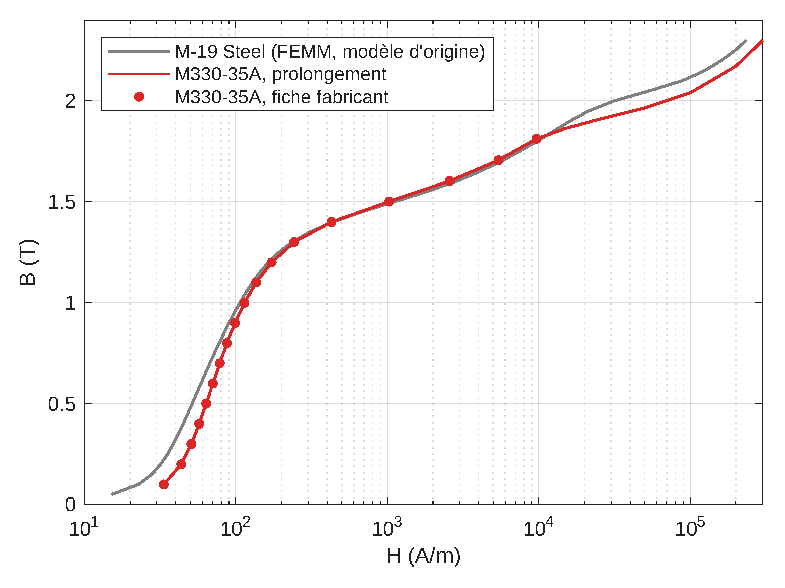
\includegraphics[width=0.62\linewidth]{figures/courbesBH}
    \caption{Courbe d'aimantation de la M330-35A (fiche du fabricant et prolongement) et de la \texttt{M-19 Steel} de FEMM utilisée auparavant.}
    \label{fig-bh}
\end{figure}

\paragraph{Coefficients de la tôle.} La même fiche donne les pertes mesurées de 50 à \SI{2500}{\hertz}. Le jeu « m330\_35a » en est tiré : $k_c = \pi^2\sigma d^2/(6\rho)$ est calculé à partir de la résistivité de la fiche et de l'épaisseur, puis $k_h$, $\alpha$ et $k_{exc}$ sont ajustés sur \eqref{eq-sinus} de 50 à \SI{400}{\hertz} et jusqu'à \SI{1.5}{\tesla}. L'écart moyen est de \SI{5}{\percent} sur les points ajustés, et de moins de \SI{1}{\percent} en moyenne à \SI{1000}{\hertz}, fréquence qui n'a pas servi à l'ajustement. Les quatre jeux comparés sont :
\begin{center}\small
\begin{tabularx}{\textwidth}{@{}lS[table-format=1.4]S[table-format=1.3]S[table-format=1.2e-1]S[table-format=1.2e-1]X@{}}
\toprule
Jeu & {$k_h$} & {$\alpha$} & {$k_c$} & {$k_{exc}$} & Origine \\
\midrule
m330\_35a & 0.0182 & 1.896 & 6.27e-5 & 7.63e-4 & tôle du prototype, ajusté sur la fiche du fabricant \cite{Sur09} \\
initial & 0.0234 & 2.33 & 5.27e-5 & 0 & M330-35A, deux points de la norme EN~10106, sans terme excédentaire \\
hugo & 0.0162 & 1.847 & 2.46e-4 & 4.11e-4 & thèse de H.~Helbling \cite{Hel21}, tôle de \SI{0.65}{\milli\metre} \\
boglietti3335 & 0.0149 & 2.11 & 9.70e-5 & 0 & tôle de \SI{0.35}{\milli\metre} de même classe \cite[table~III]{Bog03} \\
\bottomrule
\end{tabularx}
\end{center}

\paragraph{Trajectoires de courant.} Pour chaque machine, une cartographie $(i_d, i_q, \theta)$ est calculée avec xfemm (grille de 0 à \SI{20}{\ampere} par pas de \SI{1}{\ampere}, 90 positions sur un pas polaire). Les solveurs de l'article TIA de M.~Grosso, appliqués à un modèle spline de cette cartographie, donnent au couple de \SI{2}{\newton\metre} :
\begin{itemize}
    \item \textbf{P0}, MTPA du couple moyen : courant $(i_d, i_q)$ constant, le couple ondule ;
    \item \textbf{P1}, MTPA instantané : $(i_d, i_q)$ varie avec la position pour que le couple soit constant.
\end{itemize}

\paragraph{Simulation avec FEMM~5.} Chaque trajectoire est résolue position par position avec FEMM~5 (femm-qt, version 5.0.20261112, compilée localement), piloté depuis MATLAB. À chaque position : l'angle de l'élément d'entrefer est fixé, les courants des deux phases sont imposés, la résolution est lancée, puis on relève le couple (intégrale sur l'élément d'entrefer) et l'induction de tous les éléments, constante par élément et sans lissage. Le maillage est vérifié identique à toutes les positions. Les groupes des labels de bloc sont réécrits dans une copie du modèle pour reconnaître le fer du stator et du rotor.

\paragraph{Calcul des pertes.} La formule \eqref{eq-retenue} est appliquée à chaque élément ; la dérivée $\dd B/\dd t$ est calculée par transformée de Fourier sur une période, les cycles d'hystérésis par la méthode rainflow, et la somme \eqref{eq-somme} est faite sur les éléments du fer.

\paragraph{Contrôles.} En régime sinusoïdal (\SI{1.5}{\tesla}, \SI{50}{\hertz}), le calcul redonne terme à terme la formule \eqref{eq-sinus}. Sur trois positions de la trajectoire P1 de la machine à aimants (modèle d'origine en \texttt{M-19 Steel}), FEMM~5 et xfemm donnent le même couple à \SI{0.003}{\newton\metre} près, les mêmes flux de phase à \SI{0.2}{\percent} près, et la même aire de fer au stator et au rotor.

\paragraph{Fichiers.} Le dossier \texttt{pertesFer} est autonome pour le calcul des pertes : il contient les modèles, les courants, les fonctions et les scripts. Chemins relatifs à ce dossier :
\begin{center}
\begin{tabularx}{\textwidth}{@{}lX@{}}
\toprule
Fichier & Rôle \\
\midrule
\texttt{modeles/*.fem} & les deux machines, fer en M330-35A \\
\texttt{calculPertes/courants/*.csv} & courants des trajectoires P0 et P1, une ligne par position \\
\texttt{calculPertes/calculPertes.m} & simulation FEMM~5 et pertes fer ; ne lit que les courants et les modèles \\
\texttt{calculPertes/resultatsNote.m} & figures et tableaux de cette note \\
\texttt{lib/femm5Trajectoire.m} & pilotage de FEMM~5 sur une trajectoire \\
\texttt{lib/pertesFer.m} & formule \eqref{eq-retenue}, terme par terme \\
\texttt{lib/coefficientsFer.m} & jeux de coefficients \\
\texttt{lib/materiauM330\_35A.m} & données de la fiche de la tôle \\
\texttt{trajectoires/trajectoires.m} & cartographies et trajectoires P0, P1 ; demande l'environnement du projet complet (xfemm, solveurs de l'article TIA) \\
\bottomrule
\end{tabularx}
\end{center}

\section{Résultats}\label{sec-resultats}

\paragraph{Lecture.} À \SI{1500}{tr/min} et \SI{2}{\newton\metre}, fer en M330-35A (tableaux~\ref{tab-simulations} à \ref{tab-hysteresis}). Les chiffres cités sont ceux du jeu « m330\_35a », identifié sur la tôle du prototype, sauf mention contraire.
\begin{itemize}
    \item \textbf{Trajectoires.} FEMM~5 retrouve le couple de consigne à \SI{0.001}{\newton\metre} près. La loi P1 ramène l'ondulation de couple d'environ \SI{1}{\newton\metre} crête à crête (P0) à environ \SI{0.01}{\newton\metre}, au prix d'un courant qui varie avec la position.
    \item \textbf{Pertes des deux machines.} Avec la loi P1, les pertes fer valent \SI{12.6}{\watt} sans aimant et \SI{10.2}{\watt} avec aimants ; avec P0, \SI{10.8}{\watt} et \SI{7.5}{\watt}. Le stator en porte environ les trois quarts.
    \item \textbf{P1 coûte des pertes fer.} Par rapport à P0, la loi P1 augmente les pertes fer de \SI{17}{\percent} sans aimant et de \SI{37}{\percent} avec aimants (de 15 à 22 et de 29 à \SI{51}{\percent} selon le jeu). L'augmentation porte sur les termes dynamiques, sensibles aux harmoniques de courant introduits par P1.
    \item \textbf{Les aimants réduisent les pertes fer.} À couple égal et pour la loi P1, la machine à aimants a \SI{19}{\percent} de pertes fer en moins que la machine sans aimant (de 17 à \SI{26}{\percent} selon le jeu), avec un courant plus faible d'environ \SI{30}{\percent}.
    \item \textbf{Jeu de coefficients.} Le jeu « m330\_35a » donne des pertes comprises entre celles des jeux « initial » et « boglietti3335 » (\SIrange{9.3}{10.3}{\watt} sans aimant, loi P1) et celles du jeu « hugo » (\SI{18.1}{\watt}). Il se distingue par un terme excédentaire du même ordre que le terme classique (\SI{3.5}{\watt} et \SI{2.7}{\watt}), là où le jeu « hugo » met l'essentiel dans le terme classique (\SI{10.4}{\watt}). La part du rotor passe de 16 à \SI{34}{\percent} selon le jeu (\SI{27}{\percent} pour « m330\_35a ») : les pertes du rotor viennent des harmoniques d'encoches, de fréquence élevée, et dépendent donc surtout des termes dynamiques.
    \item \textbf{Hystérésis.} Le comptage des cycles et la somme sur les harmoniques diffèrent de moins de \SI{5}{\percent} (tableau~\ref{tab-hysteresis}). Au rotor, l'hystérésis reste inférieure au watt : le choix de son écriture n'a pas d'effet sensible sur le total.
    \item \textbf{Effet de la tôle sur le champ.} À coefficients égaux, remplacer la \texttt{M-19 Steel} par la M330-35A dans le calcul de champ modifie les pertes de moins de \SI{3}{\percent} (\SI{17.64}{\watt} et \SI{18.06}{\watt}, jeu « hugo », loi P1 sans aimant). L'essentiel de l'incertitude vient des coefficients de pertes, pas de la courbe B(H).
\end{itemize}


\IfFileExists{resultats.tex}{% Généré par pertesFer/calculPertes/resultatsNote.m le 17/11/2026 16:30. Ne pas éditer.
\newcommand{\vitRef}{1500}
\newcommand{\tauCons}{2}
\newcommand{\jeuCarte}{m330\_35a}
\newcommand{\nPositions}{90}
\begin{table}[H]
\centering
\caption{Trajectoires simulées avec FEMM~5 (90 positions sur un pas polaire). $I_s$ : amplitude du courant.}
\label{tab-simulations}
\resizebox{\textwidth}{!}{%
\begin{tabular}{llS[table-format=2.2]S[table-format=2.2]S[table-format=1.3]S[table-format=1.3]S[table-format=5.0]S[table-format=5.0]}
\toprule
Machine & Loi & {$I_s$ moyen (A)} & {$I_s$ max (A)} & {Couple moyen (N\,m)} & {Ondulation c-c (N\,m)} & {Éléments stator} & {Éléments rotor} \\
\midrule
sans aimant & P0 & 9.56 & 9.56 & 2.000 & 1.035 & 5107 & 8537 \\
sans aimant & P1 & 9.63 & 10.84 & 2.001 & 0.013 & 5107 & 8537 \\
avec aimants (B123\_f25) & P0 & 6.70 & 6.70 & 2.000 & 0.965 & 5107 & 8820 \\
avec aimants (B123\_f25) & P1 & 6.73 & 7.84 & 2.001 & 0.009 & 5107 & 8820 \\
\bottomrule
\end{tabular}}
\end{table}

\begin{table}[H]
\centering
\caption{Pertes fer à \SI{1500}{tr/min} et \SI{2}{\newton\metre}, machine entière (W), pour chaque jeu de coefficients.}
\label{tab-pertes}
\resizebox{\textwidth}{!}{%
\begin{tabular}{llS[table-format=2.2]S[table-format=2.2]S[table-format=1.2]S[table-format=2.2]S[table-format=2.2]S[table-format=2.2]}
\toprule
Machine & Loi & {Hystérésis} & {Classiques} & {Excédentaires} & {Stator} & {Rotor} & {Total} \\
\midrule
\multicolumn{8}{l}{\emph{Jeu « m330\_35a »}} \\
sans aimant & P0 & 5.85 & 2.03 & 2.90 & 7.70 & 3.08 & 10.78 \\
sans aimant & P1 & 6.43 & 2.65 & 3.52 & 9.14 & 3.46 & 12.60 \\
avec aimants (B123\_f25) & P0 & 4.14 & 1.29 & 2.04 & 5.75 & 1.73 & 7.48 \\
avec aimants (B123\_f25) & P1 & 4.83 & 2.27 & 3.15 & 7.88 & 2.36 & 10.24 \\
\midrule
\multicolumn{8}{l}{\emph{Jeu « initial »}} \\
sans aimant & P0 & 7.18 & 1.70 & 0.00 & 7.49 & 1.40 & 8.89 \\
sans aimant & P1 & 8.02 & 2.23 & 0.00 & 8.66 & 1.59 & 10.25 \\
avec aimants (B123\_f25) & P0 & 4.79 & 1.09 & 0.00 & 5.16 & 0.73 & 5.88 \\
avec aimants (B123\_f25) & P1 & 5.65 & 1.91 & 0.00 & 6.55 & 1.01 & 7.56 \\
\midrule
\multicolumn{8}{l}{\emph{Jeu « hugo »}} \\
sans aimant & P0 & 5.26 & 7.95 & 1.56 & 9.42 & 5.34 & 14.77 \\
sans aimant & P1 & 5.76 & 10.40 & 1.90 & 11.93 & 6.13 & 18.06 \\
avec aimants (B123\_f25) & P0 & 3.74 & 5.07 & 1.10 & 7.02 & 2.90 & 9.92 \\
avec aimants (B123\_f25) & P1 & 4.36 & 8.91 & 1.70 & 10.83 & 4.14 & 14.97 \\
\midrule
\multicolumn{8}{l}{\emph{Jeu « boglietti3335 »}} \\
sans aimant & P0 & 4.65 & 3.14 & 0.00 & 5.77 & 2.02 & 7.79 \\
sans aimant & P1 & 5.15 & 4.11 & 0.00 & 6.93 & 2.32 & 9.26 \\
avec aimants (B123\_f25) & P0 & 3.20 & 2.00 & 0.00 & 4.14 & 1.07 & 5.21 \\
avec aimants (B123\_f25) & P1 & 3.75 & 3.52 & 0.00 & 5.74 & 1.52 & 7.26 \\
\bottomrule
\end{tabular}}
\end{table}

\begin{table}[H]
\centering
\caption{Pertes par hystérésis à \SI{1500}{tr/min} (W), jeu « m330\_35a » : comptage des cycles (formule retenue) et somme sur les harmoniques (ancienne écriture).}
\label{tab-hysteresis}
\resizebox{\textwidth}{!}{%
\begin{tabular}{llS[table-format=1.2]S[table-format=1.2]S[table-format=1.2]S[table-format=1.2]}
\toprule
Machine & Loi & {Stator, cycles} & {Stator, harmoniques} & {Rotor, cycles} & {Rotor, harmoniques} \\
\midrule
sans aimant & P0 & 5.03 & 5.11 & 0.82 & 0.84 \\
sans aimant & P1 & 5.53 & 5.37 & 0.89 & 0.93 \\
avec aimants (B123\_f25) & P0 & 3.69 & 3.69 & 0.45 & 0.46 \\
avec aimants (B123\_f25) & P1 & 4.27 & 4.08 & 0.56 & 0.58 \\
\bottomrule
\end{tabular}}
\end{table}
}{\emph{Résultats non encore calculés (\texttt{calculPertes.m} puis \texttt{resultatsNote.m}).}}

\IfFileExists{figures/trajectoires.pdf}{%
\begin{figure}[H]
    \centering
    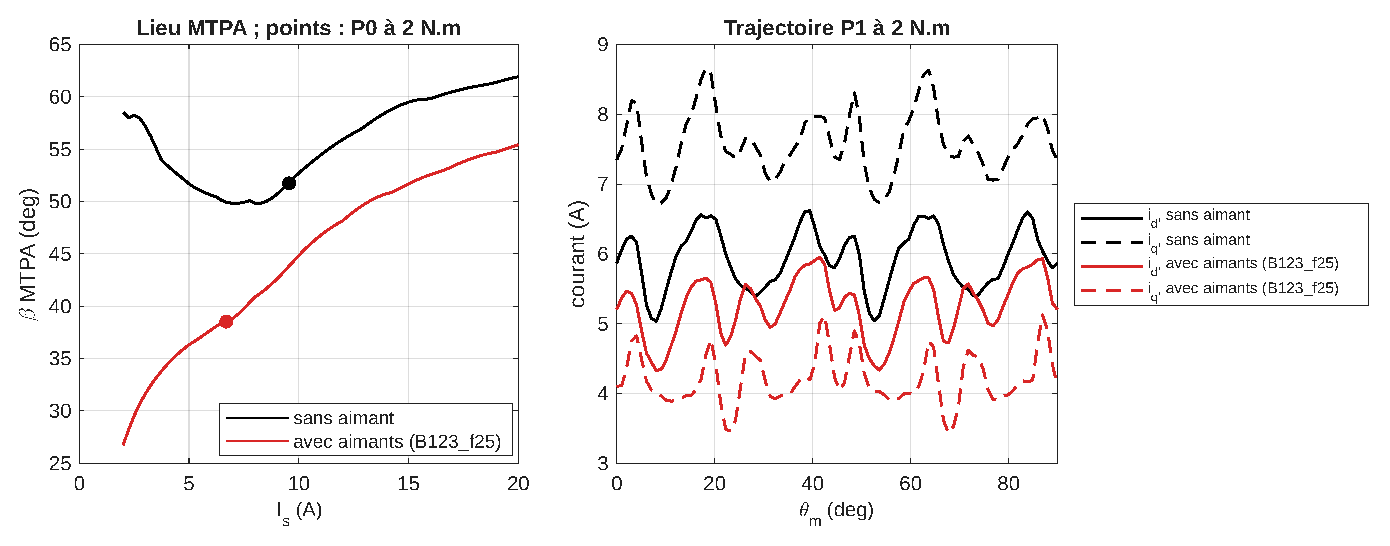
\includegraphics[width=\linewidth]{figures/trajectoires}
    \caption{Lieu MTPA et point P0 à \SI{2}{\newton\metre} (gauche) ; courants de la trajectoire P1 (droite).}
    \label{fig-trajectoires}
\end{figure}}{}

\IfFileExists{figures/pertes_vitesse.pdf}{%
\begin{figure}[H]
    \centering
    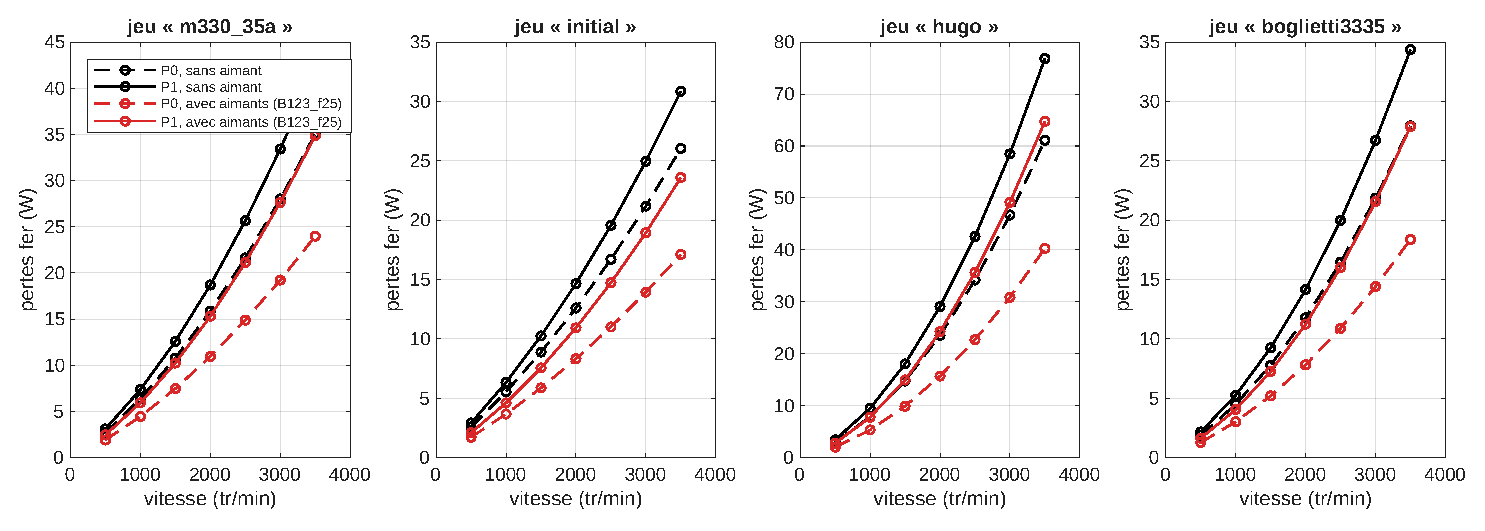
\includegraphics[width=\linewidth]{figures/pertes_vitesse}
    \caption{Pertes fer à \SI{2}{\newton\metre} en fonction de la vitesse, pour chaque jeu de coefficients ; trait plein : P1, tirets : P0.}
    \label{fig-vitesse}
\end{figure}}{}

\IfFileExists{figures/densite_pertes.pdf}{%
\begin{figure}[H]
    \centering
    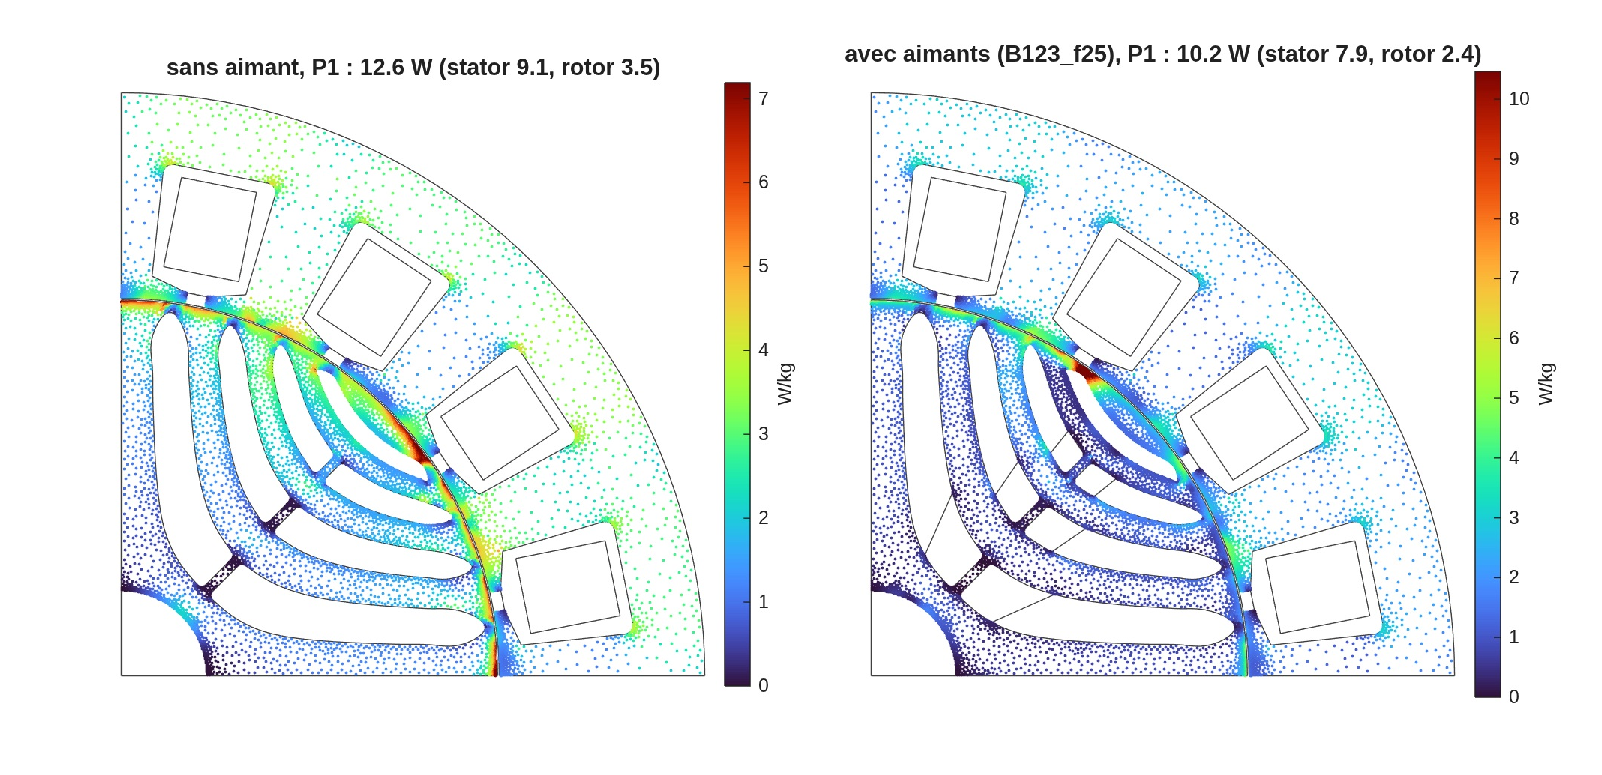
\includegraphics[width=\linewidth]{figures/densite_pertes}
    \caption{Pertes par élément (W/kg), loi P1, à \SI{1500}{tr/min}, jeu « m330\_35a ».}
    \label{fig-densite}
\end{figure}}{}

\section{Domaine de validité}

\begin{itemize}
    \item \textbf{Cycles mineurs.} La formule \eqref{eq-hyst} suppose qu'il n'y en a pas ; c'est en général le cas au stator, pas au rotor. Le comptage des cycles \eqref{eq-hyst-cycles} les prend en compte en supposant qu'un cycle mineur dissipe comme un cycle centré de même excursion, ce qui ignore le décalage dû au champ continu (section~\ref{sec-ouvert}).
    \item \textbf{Pas d'effet de peau dans la tôle.} Le terme classique suppose une induction uniforme dans l'épaisseur \cite[\S~I.1-B.3]{Hel21}. L'hypothèse se dégrade pour les harmoniques de rang élevé. Boglietti et al. proposent une correction \cite[Eq.~4]{Bog03} qui n'est pas retenue ici. Yamazaki et Fukushima comparent le modèle à trois termes à un calcul tridimensionnel des courants induits dans la tôle : les deux donnent la même précision quand les harmoniques dominants sont de rang peu élevé ou la tôle mince, mais le modèle à trois termes surestime les pertes par courants induits des harmoniques de rang élevé, et sous-estime alors l'hystérésis des cycles mineurs \cite[\S~III]{Yam10}. Rasilo et al. montrent, sur des machines synchrones à rotor bobiné dont les pôles sont en tôles épaisses, que négliger l'effet de peau et la réaction des courants induits sur le champ surestime nettement les pertes par courants induits au rotor, alors que le stator y est peu sensible \cite[\S~III-E]{Ras12}. Avec des tôles minces l'effet est moindre, mais il va dans le même sens : les pertes classiques dues aux harmoniques d'encoches au rotor sont plutôt surestimées par \eqref{eq-classique}.
    \item \textbf{Coefficients constants.} Le coefficient $k_{exc}$ est supposé indépendant de l'état d'aimantation, ce qui n'est plus vrai à forte induction ou haute fréquence \cite[\S~I.1-B.3]{Hel21}.
    \item \textbf{Champ alternatif par composante.} La somme sur $x$ et $y$ dans \eqref{eq-retenue} traite un champ tournant comme deux champs alternatifs en quadrature. Les références \cite{Fio90,Ama95,Bog03} ne traitent que le champ alternatif. Cette superposition est l'hypothèse usuelle des post-traitements de pertes fer des logiciels d'éléments finis ; elle est correcte à faible induction, se dégrade près de la saturation, et l'écart s'atténue en régime dynamique, quand les courants induits dominent \cite[\S~V.1]{Car21}. Une variante consiste à projeter l'induction sur le grand axe et le petit axe de sa trajectoire plutôt que sur $x$ et $y$ \cite[\S~V.1]{Car21}.
    \item \textbf{Plage d'identification.} Un jeu de coefficients n'est garanti que dans la plage d'induction et de fréquence où il a été ajusté.
    \item \textbf{Jeu de coefficients indissociable.} Un essai en régime sinusoïdal ne permet pas de séparer sans ambiguïté le terme classique du terme excédentaire : Boglietti et al. trouvent un terme excédentaire ajusté nul et le fondent dans le terme en $(f\Bc)^2$ \cite[\S~IV]{Bog03}. Yamazaki et Fukushima font le même constat : selon l'épaisseur de la tôle, le terme excédentaire est négligeable ou du même ordre que le terme classique, et un $k_{exc}$ identifié en négligeant l'effet de peau varie avec la fréquence et l'induction \cite[\S~II-B, Table~I et Fig.~2]{Yam10}. On ne combine donc pas le $k_c$ d'une source avec le $k_{exc}$ d'une autre, et le $k_c$ d'une tôle ne se transpose pas à une tôle d'épaisseur différente.
    \item \textbf{Ce que le modèle ne contient pas} : pertes dans les aimants, pertes mécaniques, effet des procédés de fabrication sur la tôle (découpe, compactage, qui sont l'objet de \cite{Hel21}). Ces effets ne sont pas marginaux : le poinçonnage est donné comme une cause importante de pertes supplémentaires dans \cite{Mar25}, et Boglietti et al. attribuent aux contraintes de découpe l'écart plus grand qu'ils observent sur un moteur que sur un transformateur \cite[\S~IX]{Bog03}.
\end{itemize}

\section{Points à trancher}\label{sec-ouvert}

\begin{ouvert}{Hystérésis au rotor}
Au rotor, l'induction est un champ continu auquel se superpose une ondulation. Il n'y a pas de cycle principal, seulement des cycles mineurs décalés par le champ continu. La formule \eqref{eq-hyst} ne s'applique pas, et la correction empirique de \cite{Lav78} non plus : elle corrige un cycle principal qui n'existe pas ici. Trois options :
\begin{itemize}
    \item ne compter aucune perte par hystérésis au rotor, en le disant ;
    \item traiter chaque cycle mineur comme un cycle centré de même amplitude, c'est-à-dire appliquer \eqref{eq-hyst-cycles}. C'est ce que font Yamazaki et Fukushima, qui calculent ainsi une hystérésis au rotor d'un moteur à aimants \cite[Fig.~5]{Yam10}. Quand l'ondulation se réduit à un seul harmonique de rang $n$, cette option donne $k_h\, n f_1\, B_n^{\alpha}$, comme une somme sur les harmoniques. Pour une ondulation à plusieurs harmoniques, les deux diffèrent (tableau~\ref{tab-hysteresis}) ;
    \item passer à un modèle d'hystérésis proprement dit (Preisach vectoriel dans \cite{Ras12}, modèle Play dans \cite{Car21}), ce qui sort du cadre d'une formule à coefficients.
\end{itemize}
La deuxième option est retenue dans les calculs de la section~\ref{sec-resultats}. Elle néglige l'effet du champ continu, qui augmente les pertes des cycles mineurs : elle sous-estime donc plutôt ce terme. L'enjeu reste faible, car au rotor ce sont les pertes classiques qui dominent.
\end{ouvert}


\begin{thebibliography}{10}
\bibitem{Ber88} G.~Bertotti, « General properties of power losses in soft ferromagnetic materials », \emph{IEEE Transactions on Magnetics}, vol.~24, n\textsuperscript{o}~1, p.~621--630, 1988. \emph{Eq.~2 : pertes classiques en sinusoïdal, sans effet de peau. Eq.~3 : séparation en trois termes. Eq.~9 : loi générale des pertes excédentaires. Eq.~18 et \S~IV : formule à trois termes et son domaine de validité.}

\bibitem{Fio90} F.~Fiorillo, A.~Novikov, « An improved approach to power losses in magnetic laminations under nonsinusoidal induction waveform », \emph{IEEE Transactions on Magnetics}, vol.~26, n\textsuperscript{o}~5, p.~2904--2910, 1990. \emph{Source des lois instantanées. Eq.~4 et 7 : pertes classiques. Eq.~12 et 13 : pertes excédentaires. Eq.~14 : pertes totales en non sinusoïdal. Eq.~15 : cas sinusoïdal. Eq.~16 : hystérésis.}

\bibitem{Ama95} M.~Amar, R.~Kaczmarek, « A general formula for prediction of iron losses under nonsinusoidal voltage waveform », \emph{IEEE Transactions on Magnetics}, vol.~31, n\textsuperscript{o}~5, p.~2504--2509, 1995. \emph{Mêmes expressions (Eq.~2, 3 et 10), puis approximation par le facteur de forme de la tension (Eq.~12), valable sans cycles mineurs.}

\bibitem{Bog03} A.~Boglietti, A.~Cavagnino, M.~Lazzari, M.~Pastorelli, « Predicting iron losses in soft magnetic materials with arbitrary voltage supply: an engineering approach », \emph{IEEE Transactions on Magnetics}, vol.~39, n\textsuperscript{o}~2, p.~981--989, 2003. \emph{Eq.~1 à 5 : trois termes en sinusoïdal. Eq.~4 : effet de peau. Eq.~13 et 17 : hystérésis liée à la tension moyenne redressée, courants induits à la tension efficace. Tables~III et IV : coefficients ajustés sur huit tôles.}

\bibitem{Hel21} H.~Helbling, \emph{Étude de l'impact des procédés de fabrication des machines électriques sur les propriétés des noyaux magnétiques}, thèse de doctorat, Université de Lille, 2021. \emph{\S~I.1-B.2 et I.1-B.3 : modèle de Bertotti, hypothèses et limites. Eq.~13 et 57 : formule en régime sinusoïdal. Eq.~55 : pertes classiques.}

\bibitem{Lav78} J.~D.~Lavers, P.~P.~Biringer, H.~Hollitscher, « A simple method of estimating the minor loop hysteresis loss in thin laminations », \emph{IEEE Transactions on Magnetics}, vol.~MAG-14, n\textsuperscript{o}~5, p.~386--388, 1978. \emph{Eq.~2 et 3 : correction des courants induits par les harmoniques. Eq.~4 à 6 : correction empirique de l'hystérésis pour les cycles mineurs.}

\bibitem{Car21} A.~Cariou, \emph{Contribution à la caractérisation et la modélisation des matériaux magnétiques doux pour les machines électriques en associant les modèles Play et Loss Surface (LS)}, thèse de doctorat, Université Grenoble Alpes, 2021. \emph{\S~I.2.2.2 : revue des modèles analytiques. Eq.~I-21 : Bertotti en sinusoïdal. Eq.~I-22 à I-24 : forme adaptée aux machines, avec correction des cycles mineurs. \S~V.1 : pertes en champ tournant et hypothèse de superposition.}

\bibitem{Yam10} K.~Yamazaki, N.~Fukushima, « Iron-loss modeling for rotating machines: comparison between Bertotti's three-term expression and 3-D eddy-current analysis », \emph{IEEE Transactions on Magnetics}, vol.~46, n\textsuperscript{o}~8, p.~3121--3124, 2010. \emph{Eq.~1 : modèle à trois termes appliqué aux machines, avec cycles mineurs. Eq.~3 : pertes classiques en somme d'harmoniques. \S~II-B : identification des coefficients. \S~III : comparaison avec le calcul des courants induits dans la tôle.}

\bibitem{Ras12} P.~Rasilo, A.~Belahcen, A.~Arkkio, « Importance of iron-loss modeling in simulation of wound-field synchronous machines », \emph{IEEE Transactions on Magnetics}, 2012, DOI~10.1109/TMAG.2012.2195190. \emph{Eq.~2 : terme excédentaire dans la loi de comportement. Eq.~5 : approximation classique basse fréquence. \S~III-E : effet de l'effet de peau et du couplage sur les pertes au stator et au rotor.}

\bibitem{Sur09} Surahammars Bruks (Cogent Power), \emph{Typical data for SURA\textsuperscript{\textregistered} M330-35A}, fiche technique, une page, octobre 2009, diffusée par Tata Steel : \url{https://www.tatasteeluk.com/sites/default/files/m330-35a.pdf}, consultée le 17~novembre 2026 ; copie dans \texttt{note/TataSteel\_M330-35A.pdf}. \emph{Matériau utilisé dans les modèles : courbe d'aimantation à \SI{50}{\hertz} (colonne A/m du tableau, $J$ de 0,1 à \SI{1.8}{\tesla}), pertes de 50 à \SI{2500}{\hertz} (jeu « m330\_35a »), résistivité \SI{42}{\micro\ohm\centi\metre}.}

\bibitem{Mar25} F.~Martin, A.~Belahcen, \emph{Overview of research activities}, Aalto University, Group of Electromechanics, présentation du 2~avril 2025. \emph{Effet du poinçonnage, de l'anisotropie et des contraintes sur les pertes ; modèles pour le champ tournant.}
\end{thebibliography}

\end{document}
